\documentclass[12pt,utf8,notheorems,compress,t]{beamer}
\usepackage{etex}

\usepackage{pgfpages}
\setbeameroption{show notes on second screen}
\setbeamertemplate{note page}[plain]
\newcommand{\jnote}[2]{\only<#1>{\note{\setlength\parskip{\medskipamount}\justifying\footnotesize#2\par}}}

% Workaround for the issue described at
% https://tex.stackexchange.com/questions/164406/beamer-using-href-in-notes.
\newcommand{\fixedhref}[2]{\makebox[0pt][l]{\hspace*{\paperwidth}\href{#1}{#2}}\href{#1}{#2}}

\usepackage[english]{babel}

\usepackage{mathtools}
\usepackage{booktabs}
\usepackage{stmaryrd}
\usepackage{array}
\usepackage{ragged2e}
\usepackage{multicol}
\usepackage{tabto}
\usepackage{xstring}
\usepackage{ifthen}
\usepackage[normalem]{ulem}
\usepackage[all]{xy}
\xyoption{rotate}
\usepackage{tikz}
\usetikzlibrary{calc,shapes,shapes.callouts,shapes.arrows,patterns,fit,backgrounds,decorations.pathmorphing,positioning}
\hypersetup{colorlinks=true}

\usepackage{pifont}
\newcommand{\cmark}{\ding{51}}
\newcommand{\xmark}{\ding{55}}
\DeclareSymbolFont{extraup}{U}{zavm}{m}{n}
\DeclareMathSymbol{\varheart}{\mathalpha}{extraup}{86}

\graphicspath{{images/}}

\usepackage[protrusion=true,expansion=true]{microtype}

\setlength\parskip{\medskipamount}
\setlength\parindent{0pt}

\title{A general Nullstellensatz for generalised spaces}
\author{Ingo Blechschmidt}
\date{April 11th, 2019}

\useinnertheme[shadow=true]{rounded}
\setbeamerfont{block title}{size={}}

\useinnertheme{rectangles}

\usecolortheme{orchid}
\usecolortheme{seahorse}
\definecolor{mypurple}{RGB}{150,0,255}
\setbeamercolor{structure}{fg=mypurple}
\definecolor{myred}{RGB}{150,0,0}
\setbeamercolor*{title}{bg=myred,fg=white}
\setbeamercolor*{titlelike}{bg=myred,fg=white}
\setbeamercolor{frame}{bg=black}

\usefonttheme{serif}
\usepackage[T1]{fontenc}
\usepackage{libertine}

% lifted from https://arxiv.org/abs/1506.08870
\DeclareFontFamily{U}{min}{}
\DeclareFontShape{U}{min}{m}{n}{<-> udmj30}{}
\newcommand\yon{\!\text{\usefont{U}{min}{m}{n}\symbol{'210}}\!}

\newcommand{\A}{\mathcal{A}}
\newcommand{\B}{\mathcal{B}}
\renewcommand{\C}{\mathcal{C}}
\newcommand{\M}{\mathcal{M}}
\renewcommand{\AA}{\mathbb{A}}
\newcommand{\E}{\mathcal{E}}
\newcommand{\F}{\mathcal{F}}
\renewcommand{\G}{\mathcal{G}}
\newcommand{\J}{\mathcal{J}}
\newcommand{\GG}{\mathbb{G}}
\renewcommand{\O}{\mathcal{O}}
\newcommand{\K}{\mathcal{K}}
\newcommand{\NN}{\mathbb{N}}
\newcommand{\QQ}{\mathbb{Q}}
\newcommand{\RR}{\mathbb{R}}
\newcommand{\TT}{\mathbb{T}}
\newcommand{\PP}{\mathbb{P}}
\newcommand{\ZZ}{\mathbb{Z}}
\newcommand{\CC}{\mathbb{C}}
\renewcommand{\P}{\mathcal{P}}
\newcommand{\aaa}{\mathfrak{a}}
\newcommand{\ppp}{\mathfrak{p}}
\newcommand{\fff}{\mathfrak{f}}
\newcommand{\defeq}{\vcentcolon=}
\newcommand{\defeqv}{\vcentcolon\equiv}
\newcommand{\Sh}{\mathrm{Sh}}
\newcommand{\GL}{\mathrm{GL}}
\newcommand{\Zar}{\mathrm{Zar}}
\newcommand{\op}{\mathrm{op}}
\newcommand{\Set}{\mathrm{Set}}
\newcommand{\Eff}{\mathrm{Ef{}f}}
\newcommand{\Sch}{\mathrm{Sch}}
\newcommand{\Aff}{\mathrm{Aff}}
\newcommand{\Ring}{\mathrm{Ring}}
\newcommand{\LocRing}{\mathrm{LocRing}}
\newcommand{\LRS}{\mathrm{LRS}}
\newcommand{\Hom}{\mathrm{Hom}}
\newcommand{\Spec}{\mathrm{Spec}}
\newcommand{\lra}{\longrightarrow}
\newcommand{\RelSpec}{\operatorname{Spec}}
\renewcommand{\_}{\mathpunct{.}}
\newcommand{\?}{\,{:}\,}
\newcommand{\speak}[1]{\ulcorner\text{\textnormal{#1}}\urcorner}
\newcommand{\ul}[1]{\underline{#1}}
\newcommand{\affl}{\ensuremath{{\ul{\ensuremath{\AA}}^1}}}
\newcommand{\Ll}{\text{iff}}
\newcommand{\inv}{inv.\@}
\newcommand{\seq}[1]{\mathrel{\vdash\!\!\!_{#1}}}
\newcommand{\hg}{\mathbin{:}}  % homogeneous coordinates

\setbeamertemplate{blocks}[rounded][shadow=false]

\newenvironment{indentblock}{%
  \list{}{\leftmargin\leftmargin}%
  \item\relax
}{%
  \endlist
}

% Adapted from https://latex.org/forum/viewtopic.php?t=2251 (Stefan Kottwitz)
\newenvironment<>{hilblock}{
  \begin{center}
    \begin{minipage}{9.05cm}
      \setlength{\textwidth}{9.05cm}
      \begin{actionenv}#1
        \def\insertblocktitle{}
        \par
        \usebeamertemplate{block begin}}{
        \par
        \usebeamertemplate{block end}
      \end{actionenv}
    \end{minipage}
  \end{center}}

\newcommand{\bignumber}[1]{
  \renewcommand{\insertenumlabel}{#1}\scalebox{1.5}{\usebeamertemplate{enumerate item}}
}
\newcommand{\bigheart}{
\includegraphics{heart}}

\newenvironment{changemargin}[2]{%
  \begin{list}{}{%
    \setlength{\topsep}{0pt}%
    \setlength{\leftmargin}{#1}%
    \setlength{\rightmargin}{#2}%
    \setlength{\listparindent}{\parindent}%
    \setlength{\itemindent}{\parindent}%
    \setlength{\parsep}{\parskip}%
  }%
  \item[]}{\end{list}}

\tikzset{
  invisible/.style={opacity=0,text opacity=0},
  visible on/.style={alt={#1{}{invisible}}},
  alt/.code args={<#1>#2#3}{%
    \alt<#1>{\pgfkeysalso{#2}}{\pgfkeysalso{#3}}}
}

\newcommand{\pointthis}[3]{%
  \tikz[remember picture,baseline]{
    \node[anchor=base,inner sep=0,outer sep=0] (#2) {#2};
    \node[visible on=#1,overlay,rectangle callout,rounded corners,callout relative pointer={(0.3cm,0.5cm)},fill=blue!20] at ($(#2.north)+(-0.1cm,-1.1cm)$) {#3};
  }%
}

\tikzset{
  invisible/.style={opacity=0,text opacity=0},
  visible on/.style={alt={#1{}{invisible}}},
  alt/.code args={<#1>#2#3}{%
    \alt<#1>{\pgfkeysalso{#2}}{\pgfkeysalso{#3}}}
}

\newcommand{\hcancel}[5]{%
  \tikz[baseline=(tocancel.base)]{
    \node[inner sep=0pt,outer sep=0pt] (tocancel) {#1};
    \draw[red!80, line width=0.4mm] ($(tocancel.south west)+(#2,#3)$) -- ($(tocancel.north east)+(#4,#5)$);
  }%
}

\newcommand{\explain}[7]{%
  \tikz[remember picture,baseline]{
    \node[anchor=base,inner sep=2pt,outer sep=0,fill=#3,rounded corners] (label) {#1};
    \node[anchor=north,visible on=<#2>,overlay,rectangle callout,rounded corners,callout
    relative pointer={(0.0cm,0.5cm)+(0.0cm,#6)},fill=#3] at ($(label.south)+(0,-0.3cm)+(#4,#5)$) {#7};
  }%
}

\newcommand{\explainstub}[2]{%
  \tikz[remember picture,baseline]{
    \node[anchor=base,inner sep=2pt,outer sep=0,fill=#2,rounded corners] (label) {#1};
  }%
}

\newcommand{\squiggly}[1]{%
  \tikz[remember picture,baseline]{
    \node[anchor=base,inner sep=0,outer sep=0] (label) {#1};
    \draw[thick,color=red!80,decoration={snake,amplitude=0.5pt,segment
    length=3pt},decorate] ($(label.south west) + (0,-2pt)$) -- ($(label.south east) + (0,-2pt)$);
  }%
}

% Adapted from https://latex.org/forum/viewtopic.php?t=2251 (Stefan Kottwitz)
\newenvironment<>{varblock}[2]{\begin{varblockextra}{#1}{#2}{}}{\end{varblockextra}}
\newenvironment<>{varblockextra}[3]{
  \begin{center}
    \begin{minipage}{#1}
      \begin{actionenv}#4
        {\centering \hil{#2}\par}
	\def\insertblocktitle{}%\centering #2}
        \def\varblockextraend{#3}
	\usebeamertemplate{block begin}}{
        \par
        \usebeamertemplate{block end}
        \varblockextraend
      \end{actionenv}
    \end{minipage}
  \end{center}}

\setbeamertemplate{headline}{%
  \begin{beamercolorbox}[wd=\paperwidth,ht=2.25ex]{}%
    \insertsectionnavigationhorizontal{\paperwidth}{}{}%
  \end{beamercolorbox}%
  \vskip0pt%
}

\setbeamertemplate{frametitle}{%
  \vskip0.4em%
  \leavevmode%
  \begin{beamercolorbox}[dp=1ex,center]{}%
  %   \usebeamercolor[fg]{item}{\textbf{{\Large \insertframetitle}}}
    \begin{tikzpicture}
      \def\R{8pt}
      \node (title) {\hil{\large\insertframetitle}};
      \begin{pgfonlayer}{background}
        \draw[decoration={bumps,segment length=8pt}, decorate, very thick, draw=mypurple]
          ($(title.south west) + (\R, 0)$) arc(270:180:\R) --
          ($(title.north west) + (0, -\R)$) arc(180:90:\R) --
          ($(title.north east) + (-\R, 0)$) arc(90:0:\R) --
          ($(title.south east) + (0, \R)$) arc(0:-90:\R) --
          cycle;
      \end{pgfonlayer}
    \end{tikzpicture}
  \end{beamercolorbox}%
  \vskip-0.6em%
}

\setbeamertemplate{navigation symbols}{}

\newcounter{framenumberpreappendix}
\newcommand{\backupstart}{
  \setcounter{framenumberpreappendix}{\value{framenumber}}
}
\newcommand{\backupend}{
  \addtocounter{framenumberpreappendix}{-\value{framenumber}}
  \addtocounter{framenumber}{\value{framenumberpreappendix}}
}

\newcommand{\mynav}[3]{%
  foo
}

\newcommand{\insertframeextra}{}
\setbeamertemplate{footline}{%
  \begin{beamercolorbox}[wd=\paperwidth,ht=2.25ex,dp=1ex,right,rightskip=1mm,leftskip=1mm]{}%
    % \inserttitle
    \hfill
    \insertframenumber\insertframeextra\,/\,\inserttotalframenumber
  \end{beamercolorbox}%
  \vskip0pt%
}


\newcommand{\hil}[1]{{\usebeamercolor[fg]{item}{\textbf{#1}}}}
\newcommand{\bad}[1]{\textcolor{red!90}{\textnormal{#1}}}

\begin{document}

\addtocounter{framenumber}{-1}

%\setbeamertemplate{headline}{\mynav{gray}{gray}{gray}}

{\usebackgroundtemplate{\begin{minipage}{\paperwidth}\vspace*{4.95cm}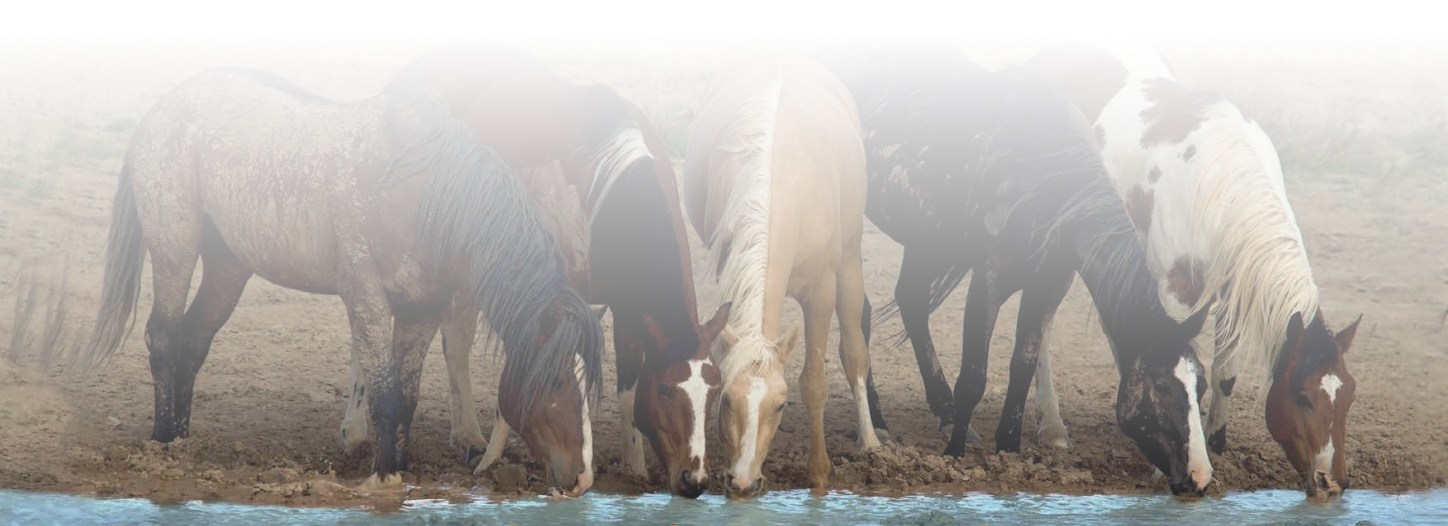
\includegraphics[width=\paperwidth]{topos-horses}\end{minipage}}
\begin{frame}[c]
  \centering

  \bigskip
  
\includegraphics[width=0.4\textwidth]{phantoms}
  \bigskip

  \begin{tikzpicture}
    \def\R{8pt}
    \node (title) {\hil{A general Nullstellensatz for generalised spaces}};
    \begin{pgfonlayer}{background}
      \draw[decoration={bumps,segment length=8pt}, decorate, very thick, draw=mypurple]
        ($(title.south west) + (\R, 0)$) arc(270:180:\R) --
        ($(title.north west) + (0, -\R)$) arc(180:90:\R) --
        ($(title.north east) + (-\R, 0)$) arc(90:0:\R) --
        ($(title.south east) + (0, \R)$) arc(0:-90:\R) --
        cycle;
    \end{pgfonlayer}
  \end{tikzpicture}

  \scriptsize
  \textit{-- an invitation --}
  \bigskip

  6th Workshop on Formal Topology in Birmingham \\
  April 11th, 2019
  \bigskip

  Ingo Blechschmidt \\
  Università di Verona
  \par

  \jnote{1}{\textcolor{red}{This set of slides will be updated soon with more
  annotations.} Right now important references are not properly mentioned, including:
  \begin{itemize}
    \item Marc Bezem, Ulrik Buchholtz and Thierry Coquand. \emph{Syntactic forcing
    models for coherent logic.}
    \item Olivia Caramello. \emph{Universal models and definability.}
    \item Carsten Butz and Peter Johnstone. \emph{Classifying toposes for
    first-order theories.}
  \end{itemize}}
\end{frame}}

{\usebackgroundtemplate{\begin{minipage}{\paperwidth}\hspace*{-1.7cm}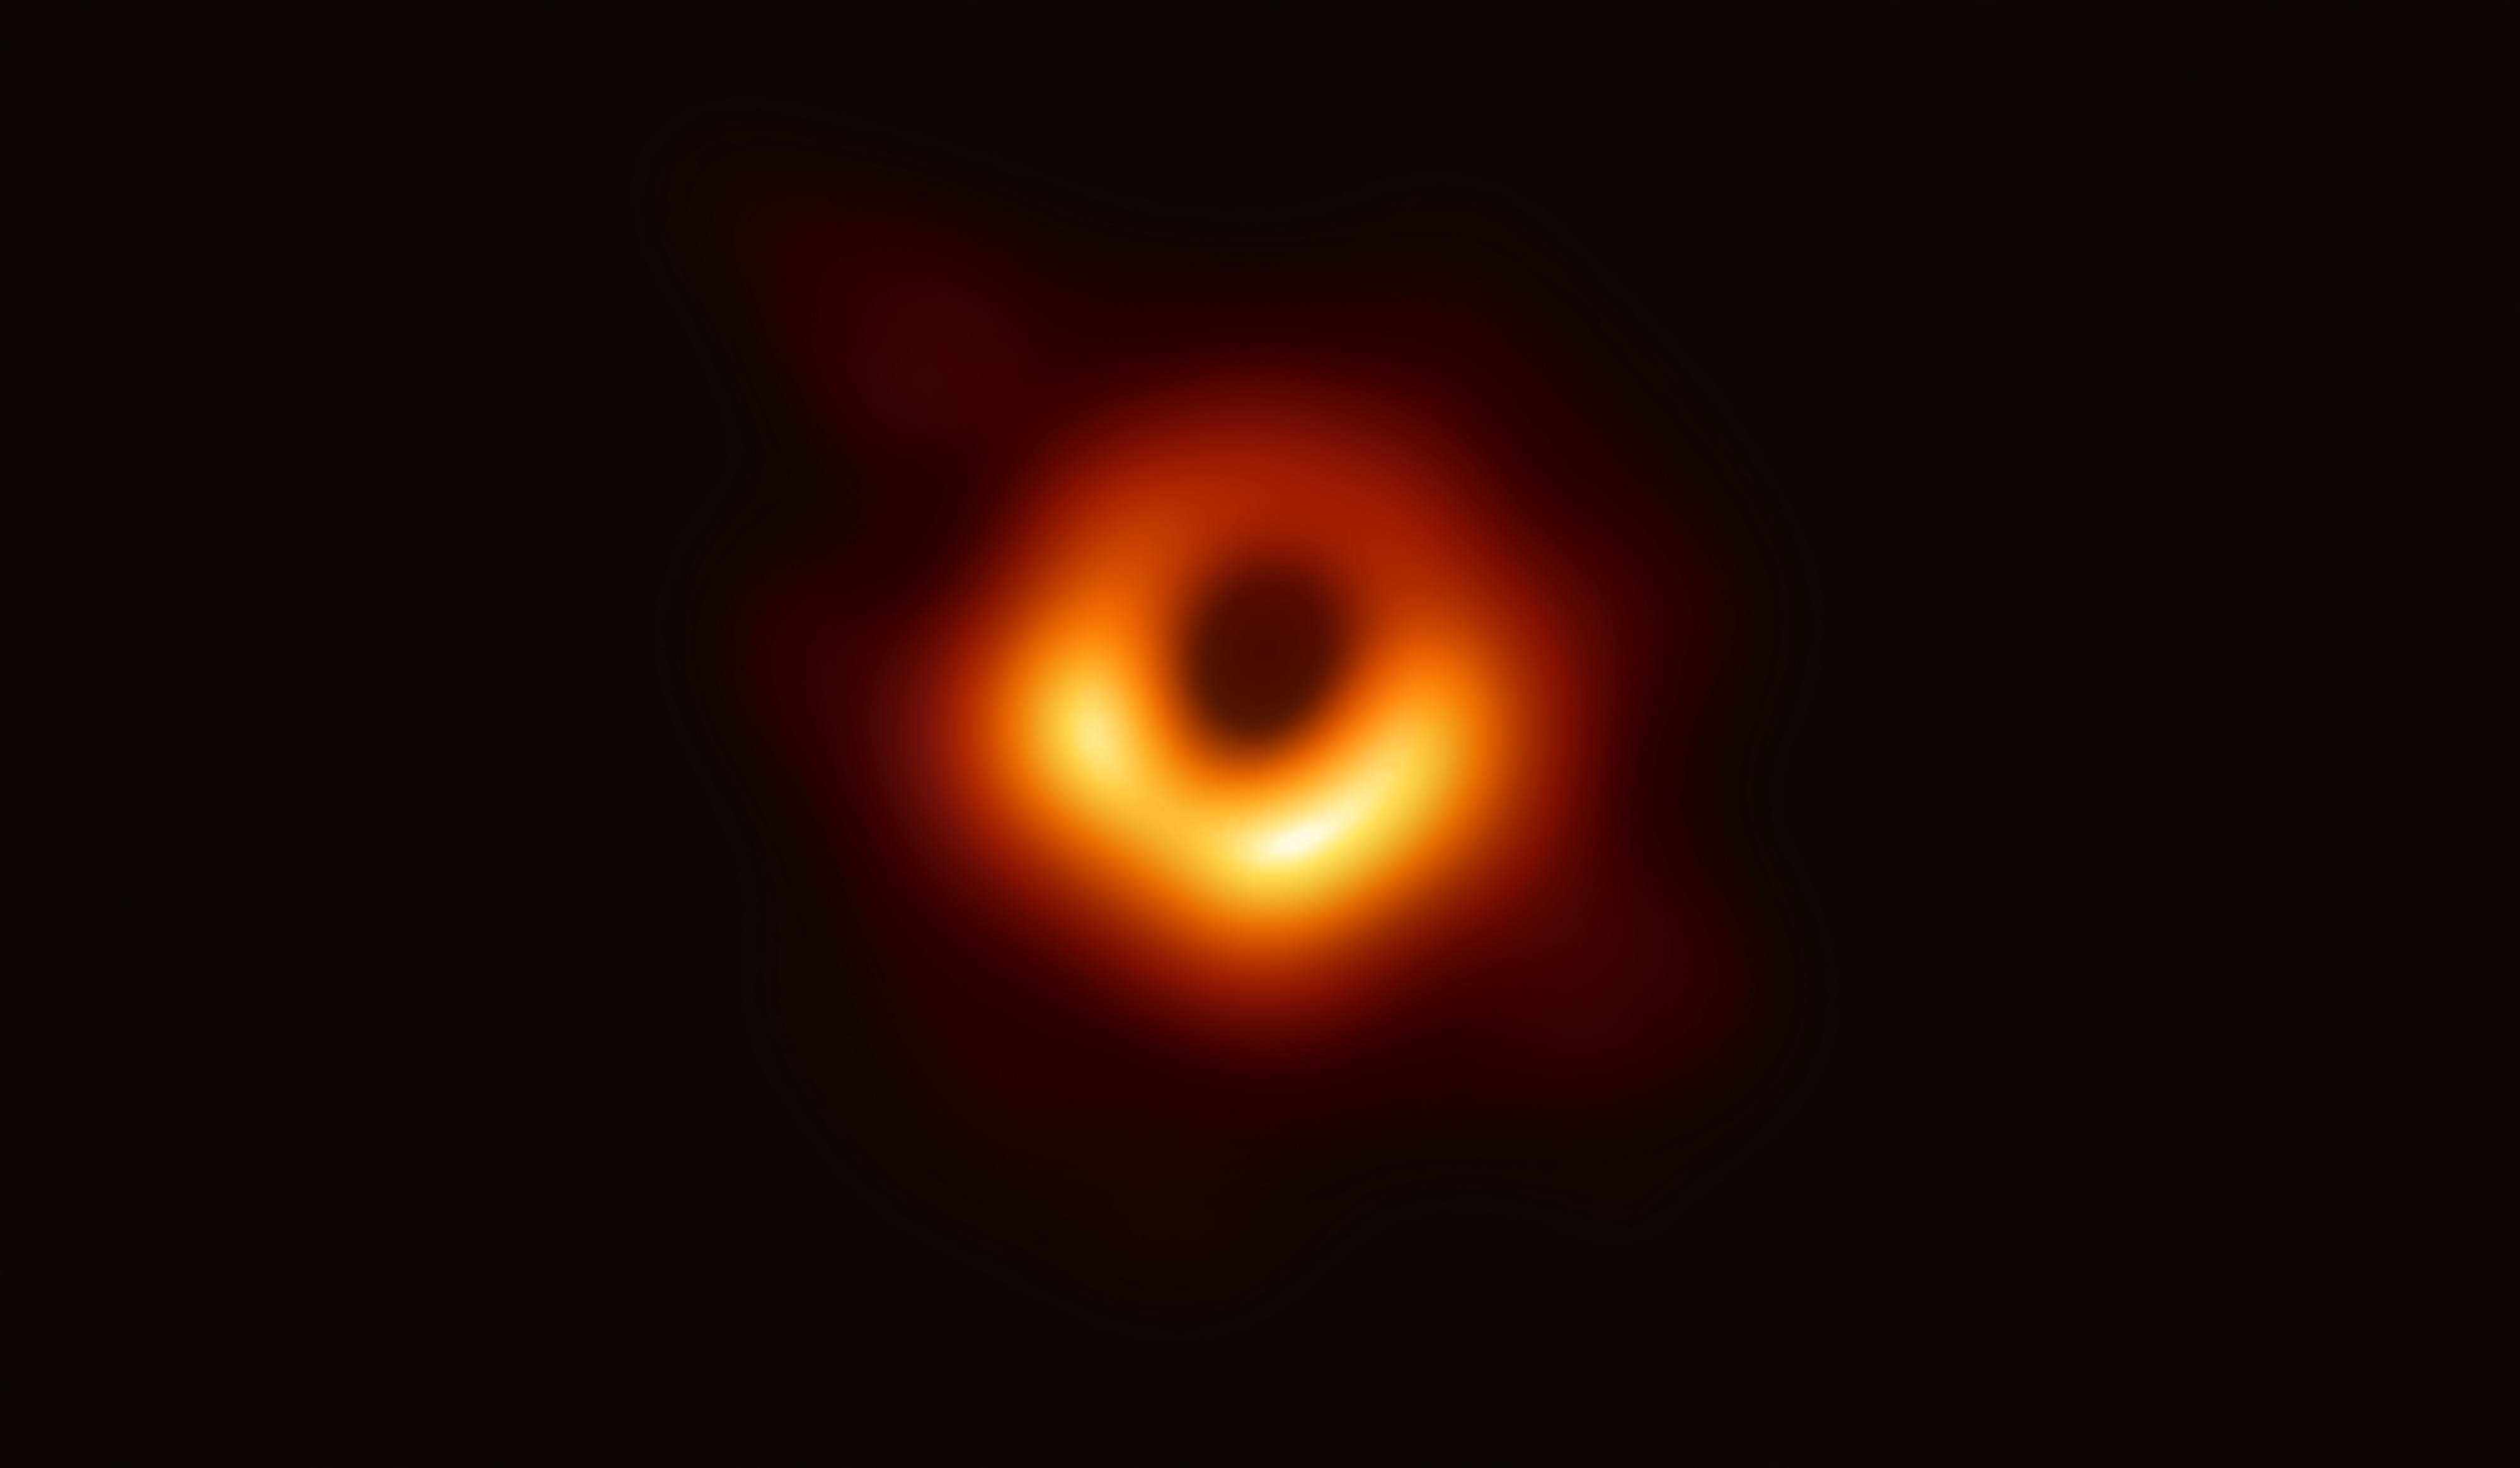
\includegraphics[height=\paperheight,trim=0 0 16.9cm 0,clip]{black-hole-m87}\end{minipage}}
\begin{frame}[plain]
  \vspace*{\paperheight}\vspace*{-0.8cm}\scriptsize
  \centering
  \textcolor{white}{Fig.: The Event Horizon Telescope picture of the central black
  hole in the galaxy M87}
  \par

  \jnote{1}{At this meeting we had lots of discussions on the notion of space.
  Here is a picture of actual space, or rather the lack thereof, released only
  yesterday.}
\end{frame}}
\addtocounter{framenumber}{-1}


\section{The generic model}

\subsection{The mystery of nongeometric sequents}

% \begin{document}

\begin{frame}{The mystery of nongeometric sequents}
  \jnote{1}{A \emph{geometric sequent} is a syntactical expression of the
  form~$(\varphi \seq{x_1\?X_1,\ldots,x_n\?X_n} \psi)$,
  where~$x_1\?X_1,\ldots,x_n\?X_n$ is a list of variable declarations,
  the~$X_i$ ranging over the available sorts, and~$\varphi$ and~$\psi$ are
  \emph{geometric formulas}. Often the variable context is abbreviated to~$\vec
  x \? \vec X$ or even just~$\vec x$. Such a sequent is read as ``in the
  context of variables~$\vec x$, $\varphi$ entails~$\psi$''.

  Geometric formulas are built from atomic propositions (using equality or the
  relation symbols) using the connectives~$\top$, $\bot$, $\wedge$, $\bigvee$
  (set-indexed disjunction) and~$\exists$. Geometric formulas may not
  contain~$\neg$, $\Rightarrow$, $\forall$.

  There is a notion of a \emph{model} of a geometric theory in
  a given topos. For instance, a ring in the usual sense is a model of the
  theory of rings in the topos~$\Set$. The structure sheaf of a scheme~$X$ is a
  model in the topos~$\Sh(X)$ of set-valued sheaves on~$X$.

  With \emph{topos} we mean Grothendieck topos, and as metatheory we use a
  constructive but impredicative flavour of English (which could be formalised
  by what is supported by the internal language of elementary toposes with an NNO).
  However the Nullstellensatz presented later makes no use of the
  subobject classifier, hence the results can likely be generalised to hold in
  a predicative metatheory or to hold for arithmetic universes.}

  \jnote{2-}{Among all models in any topos, the \emph{universal} or
  \emph{generic} one is special. It enjoys the universal property that any
  model in any topos can be obtained from it by pullback along an essentially
  unique geometric morphism. It is intriguing from a logical point of view
  because it has exactly those properties which are shared by any model in any
  topos.

  One could argue, with a certain amount of success, that the generic model of
  the theory of rings is what a mathematician implicitly refers to when she
  utters the phrase ``Let~$R$ be a ring''. This point of view is fundamental to
  the slogan \emph{continuity is geometricity}, as expounded for instance in
  \fixedhref{http://www.cs.bham.ac.uk/~sjv/GeoAspects.pdf}{Continuity and
  geometric logic} by Steve Vickers.}

  \jnote{3-}{Crucially, the conservativity statement only pertains to
  properties which can be put as geometric sequents. Generic models may have
  additional nongeometric properties. Because conservativity does not apply to
  them, they are not shared by all models in all toposes -- but any consequences
  which can be put as geometric sequents are.

  For instance, if we want to verify a geometric sequent for all local rings,
  we may freely use the displayed field axiom.
  Hence one reason why these nongeometric sequents are interesting is because
  they provide us with new reduction strategies (``without loss of
  generality'').}

  Let~$\TT$ be a \explain{geometric theory}{1-}{red!20}{-1cm}{0cm}{0cm}{\begin{minipage}{4.3cm}
    \small
    sorts,
    function symbols,
    relation symbols,
    geometric sequents as axioms
  \end{minipage}}, for instance the
  \explain{theory of rings}{1-}{blue!20}{-1cm}{0cm}{0cm}{\begin{minipage}{4.3cm}
    \small
    \begin{tabbing}
      fun. symb.: \= \kill
      sorts: \> $R$ \\
      fun. symb.: \> $0$, $1$, $-$, $+$, $\cdot$ \\
      % rel. symb.: \> \emph{none} \\
      axioms: \> $(\top \vdash_{x,y:R} x y = y x)$, \ldots
    \end{tabbing}
  \end{minipage}}.

  \vspace*{1.8cm}

  \begin{center}
    \begin{tikzpicture}[ultra thick, node distance=7mm]
      \node[rectangle, rounded corners=1pt, draw=lime!80, fill=lime!40] (a) {$\ZZ$};
      \node[rectangle, rounded corners=1pt, draw=lime!80, fill=lime!40, right=of a] (b) {$\ZZ[X,Y,Z]/(X^n+Y^n-Z^n)$};
      \node[regular polygon, regular polygon sides=5, draw=orange!80,
      fill=orange!20, right=of b, rounded corners=1pt, inner sep=0cm] (c) {$\O_X$};
      \node[star, rounded corners=1pt, star points=10, inner sep=0cm, draw=purple!80, fill=purple!20, right=of c] {$U_\TT$};
    \end{tikzpicture}
  \end{center}

  \vspace*{-0.5cm}
  \pause

  \justifying
  \textbf{Theorem.} There is a \hil{generic model}~$U_\TT$. It is
  \hil{conservative} in that
  for any \explainstub{geometric sequent}{yellow!70}~$\sigma$ the following notions coincide:
  \vspace*{-1.2em}
  \begin{enumerate}
    \item The sequent~$\sigma$ holds for~$U_\TT$.
    \item The sequent~$\sigma$ holds for any~$\TT$-model in any
    \explainstub{topos}{purple!20}.
    \item The sequent~$\sigma$ is provable modulo~$\TT$.
  \end{enumerate}

  \pause

  \justifying
  %\textbf{Main observation.} The generic model can validate nongeometric
  %sequents which are not provable modulo~$\TT$ and which do not hold for
  %arbitrary models in arbitrary toposes.

  \textbf{Observation (Kock).} The generic local ring is a field:
  \vspace*{-0.2cm}
  \[ (x = 0 \Rightarrow \bot) \vdash_{x:R} (\exists y\?R\_ xy = 1) \]
\end{frame}


\subsection{Construction of the generic model}

\begin{frame}{Construction of the generic model}
  The generic model is \hil{not} the same as \ldots
  \begin{itemize}
    \item the \hil{initial model} (think~$\ZZ$) or
    \item the \hil{free model on one generator} (think~$\ZZ[X]$).
  \end{itemize}
  Set-based models are \hil{too inflexible}.

  \textbf{Definition.} The \hil{syntactic site}~$\C_\TT$ has \ldots
  \begin{enumerate}
    \item objects: $\{ x_1\?X_1, \ldots, x_n\?X_n\_ \varphi \}$ (shorter:
    $\{ \vec x\_ \varphi \}$)
    \item morphisms: eqv. classes of \explainstub{provably functional
    formulas}{red!20}
    \item coverings: \explainstub{provably jointly surjective
    families}{purple!30}
  \end{enumerate}
  The topos of sheaves over~$\C_\TT$ is the \hil{classifying
  topos}~$\Set[\TT]$. The generic model interprets a sort~$X$ by~$\yon\{x\?X\_\top\}$.

  \jnote{1}{In case the theory~$\TT$ is a Horn theory (for instance if it is
  an equational theory), the \emph{term algebra} (the set of terms in the
  empty context modulo provable equality) is a model of~$\TT$. While such
  models do enjoy some nice categorical properties, they are in general
  \emph{not} the generic model.

  For instance, if~$\TT$ is the theory of rings, then the initial model
  is~$\ZZ$. This model validates some geometric sequents which are not
  validated by all rings, for instance~$(x^2 = 0 \seq{x:R} x = 0)$ or $(1 = 0
  \vdash \bot)$.

  In general, the generic model cannot be realised as a set-based model (with
  a set for each sort, a map for each function symbol and so on). Sets are too
  constant for this purpose; the flexibility of sheaves (``variable sets'') is
  required: The generic model lives in the topos of set-valued
  sheaves over~$\C_\TT$.}

  \jnote{2}{A morphism~$A = \{\vec x\_ \varphi\} \to \{\vec y\_ \psi\} = B$ in~$\C_\TT$ is the
  equivalence class (modulo provable equivalence) of a geometric
  formula~$\theta$ such that~$\TT$ proves
  \begin{enumerate}
    \item ``$\theta$ is a relation on~$A \times B$'': $(\theta \seq{\vec x,
    \vec y} \varphi \wedge \psi)$
    \item ``$\theta$ is total'': $(\varphi \seq{\vec x} \exists \vec y\_
    \theta)$
    \item ``$\theta$ is single-valued'': $(\theta \wedge \theta[\vec y'/\vec y]
    \seq{\vec x,\vec y,\vec y'} \vec y = \vec y')$
  \end{enumerate}

  \vspace*{-0.6em}
  A family~$(\{ \vec x_i\_ \varphi_i \} \xrightarrow{[\theta_i]} \{ \vec y\_
  \psi \})_i$ is a covering iff~$\TT$ proves~$(\psi \seq{\vec y} \bigvee_i
  \exists \vec x_i\_ \theta_i)$.

  The slides experiment with using the symbol~``$\yon$'' for the Yoneda
  embedding~$\C_\TT \to \Set[\TT]$, as in \fixedhref{http://www.math.jhu.edu/~eriehl/elements.pdf}{Elements
  of~$(\infty,1)$-category theory} by Emily Riehl and Dominic Verity.}

  \jnote{3}{The special case that the generic model of a theory~$\TT$ can be realised as
  a model in~$\Set$ occurs iff~$\TT$ is Morita-equivalent to the
  empty theory, that is, iff~$\TT$ has exactly one model in any topos.

  The special case that there exists at least some conservative~$\TT$-model
  in~$\Set$ occurs iff~$\TT$ has a conservative geometric expansion to a theory
  which is Morita-equivalent to the empty theory.}
\end{frame}


\subsection{Going internal}

\begin{frame}{Working internally to toposes}
  \justifying
  Let~$\C$ be a site. We recursively define
  \[
    U \models \varphi \quad
    \text{(``$\varphi$ holds on~$U$'')}
  \]
  for objects~$U \in \C$ and \squiggly{formulas}~$\varphi$.
  Write~``$\Sh(\C) \models \varphi$'' for~$1 \models \varphi$.
  \footnotesize
  \[ \renewcommand{\arraystretch}{1.08}\begin{array}{@{}l@{\ \ }c@{\ \ }l@{}}
  U \models \top &\Ll& \text{true} \\
  U \models \bot &\Ll& \hcancel{\text{false}}{0pt}{3pt}{0pt}{-2pt}\ \text{the
  empty family is a covering of~$U$} \\
  U \models s = t \? F &\Ll& s|_U = t|_U \in F(U) \\
  U \models \varphi \wedge \psi &\Ll&
  \text{$U \models \varphi$ and $U \models \psi$} \\
  U \models \varphi \vee \psi &\Ll&
  \hcancel{\text{$U \models \varphi$ or $U \models
  \psi$}}{0pt}{3pt}{0pt}{-2pt}\ \text{there exists a covering $(U_i \to U)_i$} \\
  && \quad\quad\text{such that for all~$i$: $U_i \models \varphi$ or $U_i \models \psi$} \\
  U \models \varphi \Rightarrow \psi &\Ll&
  \text{for all~$V \to U$: }
  \text{$V \models \varphi$ implies $V \models \psi$} \\
  U \models \forall s \? F\_ \varphi(s) &\Ll&
  \text{for all $V \to U$ and sections~$s_0 \in F(V)$: $V \models \varphi(s_0)$} \\
  % U \models \forall F\_ \varphi(F) &\Ll&
  % \text{for all $V \to U$ and sheaves~$F_0$ over~$V$: $V \models \varphi(F_0)$} \\
  U \models \exists s \? F\_ \varphi(s) &\Ll&
  \hcancel{\text{there exists $s_0 \in F(U)$ such that $U \models \varphi(s_0)$}}{0pt}{3pt}{0pt}{-2pt} \\
  &&
  \text{there exists a covering $(U_i \to U)_i$ such that for all~$i$:} \\
  && \quad\quad \text{there exists~$s_0 \in F(U_i)$ such that $U_i \models \varphi(s_0)$}
  %U \models \exists F\_ \varphi(F) &\Ll&
  %\hcancel{\text{there exists a sheaf $F_0$ on $U$ such that $U \models
  %\varphi(F_0)$}}{0pt}{3pt}{0pt}{-2pt} \\
  %&&
  %\text{there exists a covering $(U_i \to U)_i$ such that for all~$i$:} \\
  %&& \quad\quad \text{there exists a sheaf~$F_0$ on $U_i$ such that $U_i \models \varphi(F_0)$}
  \end{array} \]

  \jnote{1}{
    The internal language of a (Grothendieck or elementary) topos~$\E$ is a
    device which allows us to speak and reason about the objects and morphisms
    of~$\E$ in a naive element-based language close to the usual formal
    mathematical language. Using this language, objects of~$\E$ look like plain
    old sets [or types]; morphisms look like plain old maps between those sets;
    epimorphisms look like surjections; group objects look like groups; and so on.

    In particular, we can use the internal language to define what it means for a
    given~$\TT$-structure in~$\E$ to be a model -- namely iff it looks like a
    model from the internal point of view.

    The internal language can be implemented by the \emph{Kripke--Joyal semantics},
    a translation procedure which converts formulas of the internal language
    into external statements about the objects and morphisms of~$\E$. The slide
    displays some of the translation rules in the case that~$\E$ is a
    Grothendieck topos.

    We can actually do mathematics internally because the Kripke--Joyal
    semantics is sound with respect to intuitionistic logic: If~$\E \models
    \varphi$ and if~$\varphi$ intuitionistically entails a further
    formula~$\psi$, then~$\E \models \psi$.

    An instructive special case is provided by the topos~$\Set$, because~$\Set
    \models \varphi$ iff~$\varphi$ holds in the usual mathematical sense.
  }

  \jnote{2}{
    The Kripke--Joyal semantics can be extended to interpret unbounded
    quantification (``for all sets'' as opposed to ``for all elements of the
    particular set~$X$'') and dependent types. The former are for instance
    required to express universal properties (``for all groups'', ``for all
    rings''), and the latter are all over the place, even if their use might
    not be particularly highlighted.

    With these extensions, we can
    import all of everyday constructive impredicative mathematics into the
    internal world of a topos.

    Some illustrations of working with the internal language can be found in these
    sets of slides:
    \begin{itemize}
      \item
      \fixedhref{https://rawgit.com/iblech/internal-methods/master/slides-leipzig2018.pdf}{Slides
      for Jürgen Jost's group seminar at the MPI Leipzig}
      \item
      \fixedhref{https://rawgit.com/iblech/internal-methods/master/slides-como2018.pdf}{Slides
      for \emph{Toposes in Como}}
      (recording
      \fixedhref{https://www.youtube.com/watch?v=SuELfC5P_R8}{available})
    \end{itemize}
    A longer exposition, with pointers to the literature, can be found in Section~2 of
    \fixedhref{https://rawgit.com/iblech/internal-methods/master/notes.pdf}{these notes}.
  }
\end{frame}


\section[Nongeometric properties]{A selection of nongeometric properties}

\begin{frame}{A selection of nongeometric properties}
  The \hil{generic object} validates:
  \begin{enumerate}
    \item $\forall x,y\?U_\TT\_ \neg\neg(x = y)$.
    \item $\forall x_1,\ldots,x_n\?U_\TT\_ \neg \forall y\?U_\TT\_
    \bigvee_{i=1}^n y = x_i.$
    \item $(U_\TT)^{U_\TT} \cong 1 \amalg U_\TT$.
  \end{enumerate}

  The \hil{generic ring} validates:
  \begin{enumerate}
    \item $\forall x\?U_\TT\_ \neg\neg(x = 0)$.
    \item $\forall x\?U_\TT\_ (x = 0 \Rightarrow 1 = 0) \Rightarrow (\exists
    y\?U_\TT\_ xy = 1)$.
  \end{enumerate}

  The \hil{generic local ring} validates:
  \begin{enumerate}
    \item $\neg \forall x\?U_\TT\_ \neg\neg(x = 0)$.
    \item $\forall a_0,\ldots,a_{n-1}\?U_\TT\_ \neg\neg \exists x\?U_\TT\_
      x^n + a_{n-1}x^{n-1} + \cdots + a_0 x^0 = 0$.
    \item \justifying Let~$\Delta = \{ \varepsilon \? U_\TT \,|\, \varepsilon^2 = 0 \}$.
    For any map~$f : \Delta \to U_\TT$, there are unique elements~$a,b \?
    U_\TT$ s.\,th.~$f(\varepsilon) = a + b\varepsilon$ for all~$\varepsilon
    \? \Delta$.
%   \item For any finitely presented~$U_\TT$-algebra~$A$,
%   the canonical map~$A \to (U_\TT)^{\Hom_{U_\TT}(A,U_\TT)}$
%   is an isomorphism.
  \end{enumerate}

  \jnote{1}{
    The generic object, the generic model of the theory which has exactly one
    sort and no function symbols, relations symbols or axioms, appears to be
    slightly indecisive: On the one hand, up to a double negation, it is a
    subsingleton; on the other hand, it is infinite. This observation is due to
    Carsten Butz and Peter Johnstone
    (\fixedhref{http://citeseerx.ist.psu.edu/viewdoc/download?doi=10.1.1.16.4102&rep=rep1&type=pdf}{Classifying toposes for
    first-order theories}).

    The generic ring, the generic model of the theory of rings, is similarly
    indecisive. It is infinite in the following sense:
    \[ \forall x_1,\ldots,x_n \? U_\TT\_
      \bigl(\forall y \? U_\TT\_ \bigvee_{i=1}^n (y = x_i)\bigr) \Rightarrow
      1 = 0. \]

    The theory of local rings is the quotient theory of the theory of rings
    obtained by adding the axioms~$(1 = 0 \vdash \bot)$ and~$((\exists z\_
    (x+y)z = 1) \seq{x,y} (\exists z\_ xz = 1) \vee (\exists z\_ yz = 1))$.
    (Assuming the Boolean prime ideal theorem, a ring is local in this sense
    iff it local in the usual sense (has exactly one maximal ideal).)

    The first displayed property of the generic local ring illustrates
    that nongeometric sequents need not be inherited by quotient theories.
  }

  \jnote{2}{
    All of the displayed properties give rise to reduction techniques:
    If we want to verify a geometric sequent for all rings, it suffices to
    verify it for the generic ring; but the generic ring has additional
    nongeometric properties not shared by every ring, such as the two displayed
    ones. (This was for instance used
    \fixedhref{https://www.sciencedirect.com/science/article/pii/0022404976900025}{by
    Anders Kock} and
    \fixedhref{https://link.springer.com/chapter/10.1007\%2FBFb0061835}{by
    Gonzalo Reyes}.)

    However, we face some challenges when pursuing these reduction techniques, including
    the following:
    \begin{enumerate}\justifying
      \item It is not easy to determine interesting and useful properties of
      the generic model.
      \item The set of validated nongeometric sequents changes slightly
      unpredictably when passing to quotient theories. For instance, when
      proving that a geometric sequent holds for all rings, we may assume that
      any element is \emph{not not} zero. But we may not assume this
      simplification if we want to verify a geometric sequent for all local
      rings (and if we want to exploit the given locality in the proof).
      \item There is only so much we want to state and prove in full generality
      for all rings, all local rings, all modules, and so on. We are often much
      more interested in properties of particular mathematical objects.
    \end{enumerate}
  }

  \jnote{3}{
    The firstly-mentioned problem on the previous page is alleviated by the
    Nullstellensatz presented in this talk, which gives a systematic and
    universal source of nongeometric sequents validated by the generic model.
    However, manual work is still required to reduce this set of sequents to a
    smaller, manageable one consisting of memorable properties while hopefully
    still preserving universality.

    To counter the third problem, it's prudent to consider geometric theories
    which depend on a given mathematical object of interest. For instance,
    given a ring~$A$, we can consider the theory of prime ideals of~$A$, of
    complemented prime ideals, of filters, and so on. The classifying toposes
    of these theories are of independent interest -- in fact they are sheaf
    toposes over certain important spaces in algebraic geometry -- and
    nongeometric sequents validated by their generic models bundle nontrivial
    information about~$A$. More details are on the following slide.
  }
\end{frame}


\section{Affine schemes}

\begin{frame}{Affine schemes}
  \jnote{1}{
    A ring is \emph{local} iff every invertible sum contains an invertible
    summand, that is if~$1 \neq 0$ and if~$x + y$ invertible implies~$x$
    invertible or~$y$ invertible. Assuming the axiom of choice, this elementary
    definition is equivalent to the textbook definition of a local ring (a ring
    with exactly one maximal ideal). A ring homomorphism is \emph{local} iff it
    reflects invertibility.

    The notion of a \emph{filter} in a ring~$A$ is a direct axiomatisation of
    what classically would be the complement of a prime ideal. The filter
    axioms are: $1 \in F$, $(xy \in F) \Leftrightarrow ((x \in F) \wedge (y \in
    F))$, $\neg(0 \in F)$, $(x+y \in F) \Rightarrow ((x \in F) \vee (y \in F))$.

    A \emph{free local ring} over~$A$ is a homomorphism into a local
    ring~$A'$ such that any homomorphism into a local ring~$R$ factors uniquely
    over~$A'$ via a local homomorphism.

    For any particular local ring~$A \xrightarrow{f} R$, the
    localisation~$A[S^{-1}]$ with~$S = f^{-1}[R^\times]$ is a local ring which
    fits into the displayed diagram. However, in general there is no single
    choice of~$S$ which would work for any local ring~$R$. Indeed, classically
    one can show that a free local ring over~$A$ exists if and only if~$A$
    contains exactly one prime ideal, in which case~$A$ itself is the free
    local ring.
  }

  \jnote{2}{
    If we want a free local ring to exist for any ring~$A$, we have to broaden
    our notion of existence and embrace rings which live in toposes other
    than~$\Set$. There is a notion of a homomorphism between rings living in
    arbitrary toposes, and using this notion one can verify:

    The free local ring over~$A$ can be built in the classifying topos of
    filters of~$A$, as the localisation (in that topos) of~$A$ at the generic
    filter. (More precisely, as the localisation of the mirror image of~$A$ in that
    topos, that is the constant sheaf~$\underline{A}$.)

    The classifying topos of filters of~$A$ coincides with the topos of sheaves
    over what's called the \emph{spectrum of~$A$} in algebraic geometry, and
    under this equivalence the free local ring coincides with the structure
    sheaf of spectrum. In fact the classifying topos serves as a good
    constructive substitute for the classical spectrum construction,
    enjoying the expected universal property even if the axiom of choice is not
    available, which is why it is simply denoted~``$\Spec(A)$'' on the slide.

    (The classifying topos of prime ideals of~$A$ is also interesting; it
    coincides with the topos of sheaves over the spectrum of~$A$ equipped with
    the constructible topology.)
  }

  \jnote{3}{
    Assuming the Boolean prime ideal theorem, the geometric sequents
    validated by~$A^\sim$ are easy to describe: They are precisely those which
    are validated by all the stalks~$A_\ppp$ of~$A$.

    But~$A^\sim$ enjoys further unique properties which are not shared by the
    stalks of~$A$, other localisations of~$A$, quotients of~$A$ or indeed any
    reasonable construction. Three of these are displayed on the slide.
    (A ring is \emph{anonymously Noetherian} iff each of its ideals is
    \emph{not not} finitely generated. Textbook proofs of Hilbert's basis theorem
    are constructively acceptable for this Noetherian condition.)

    The object~$A^\sim$ strikes a fine balance: On the one hand, it is still
    close to~$A$, so that information learned about~$A^\sim$ teaches us
    about~$A$; on the other hand, it enjoys unique properties rendering it
    simpler than~$A$.

    This balance allows for a simple and conceptually satisfying proof of
    \emph{Gro\-then\-dieck's generic freeness lemma}, an important theorem in
    algebraic geometry. Details can be found in
    \fixedhref{https://rawgit.com/iblech/internal-methods/master/slides-padova2018.pdf}{this
    set of slides}.
  }

  Let~$A$ be a ring. Is there a \hil{free local ring}~$A \to A'$ over~$A$?
  \begin{columns}[t]
    \begin{column}{0.4\textwidth}
      $\xymatrix{
        A \ar[rd] \ar[rrr]^f &&& {\substack{\phantom{\text{local}}\\\text{\normalsize$R$}\\\text{local}}} \\
        & {\substack{\text{\normalsize$A'$}\\\text{local}}} \ar@{-->}_[@!35]{\text{local}}[rru]
      }$
    \end{column}

    \begin{column}{0.50\textwidth}
      \small\justifying
      For a fixed ring~$R$, the localisation $A' \defeq A[S^{-1}]$ with $S \defeq
      f^{-1}[R^\times]$ would do the job. ($S$ is a \emph{filter}.)
      \medskip

      Hence we need the \hil{generic filter}.
    \end{column}
  \end{columns}

  \pause

  \justifying
  The free local ring over~$A$ is~$A^\sim \defeq \ul{A}[F^{-1}]$,
  where~$F$ is the generic filter, living in~$\Spec(A)$, the classifying topos
  of filters of~$A$.

  \pause

  If~$A$ is reduced ($x^n = 0 \Rightarrow x = 0$):

  \vspace*{-0.8em}
  \setbeamercolor{block body}{bg=red!30}
  \setbeamercolor{structure}{fg=purple}
  \begin{varblock}{\textwidth}{}
    $A^\sim$ is a \hil{field}: $\forall x\?A^\sim\_ (\neg(\exists y\?A^\sim\_
    xy = 1) \Rightarrow x = 0)$.

    $A^\sim$ has \hil{$\boldsymbol{\neg\neg}$-stable equality}:
    $\forall x,y\?A^\sim\_ \neg\neg(x = y) \Rightarrow x = y$.

    \mbox{$A^\sim$ is \hil{anonymously Noetherian}.}\\[-1.2em]
  \end{varblock}
\end{frame}


\section[A systematic source]{A systematic source of nongeometricity?}

\begin{frame}{A systematic source of nongeometricity?}
  \jnote{1-2}{
    Mimicking the synthetic approach to differential geometry, synthetic
    algebraic geometry is a framework for algebraic geometry in which schemes
    can be modelled by plain old sets, morphisms of schemes by plain old maps
    between those sets, group schemes by plain old groups, and so on. Unlike
    its close cousin, it is far less developed; some first steps are outlined
    in Sections~19 and~20 of
    \fixedhref{https://rawgit.com/iblech/internal-methods/master/notes.pdf}{these notes}.

    Synthetic algebraic geometry is carried out internally to the \emph{big
    Zariski topos} of a given base scheme; in the special case that the base
    scheme is the terminal scheme~$\Spec(\ZZ)$, this topos is just the
    classifying topos of local rings. The relevant generic model living in the
    big Zariski topos is denoted~``$\affl$'' because it coincides with the
    functor of points of the affine line.
  }

  \jnote{2}{
    Marc Bezem, Ulrik Buchholtz and Thierry Coquand answered in their 2017 paper
    \fixedhref{https://arxiv.org/abs/1712.07743}{Syntactic forcing
    models for coherent logic} Gavin Wraith's question in the negative. (As
    Thierry remarked during the talk, this is even if one takes care to phrase
    the question in a way to exclude the trivial counterexamples given by
    instances of the law of excluded middle in the language of~$\TT$.) If the
    answer had been positive, this would have given a neat, if somewhat hard to
    use in practice, characterisation of the formulas validated by the generic model.
  }

  \jnote{3}{
    The topos-theoretic \emph{Nullstellensatz}, to be presented on the next
    slides, answers the displayed three questions in the affirmative.

    Briefly, the Nullstellensatz is a certain statement in the language of a
    given geometric theory~$\TT$ which is
    \begin{itemize}\justifying
      \item validated by the generic~$\TT$-model,
      \item typically not validated by other~$\TT$-models, and
      \item such that any statement validated by the generic~$\TT$-model can be
      deduced, in intuitionistic logic, from the axioms of~$\TT$ and the
      Nullstellensatz.
    \end{itemize}

    We believe that this characterisation is as explicit as it can get, but
    would be delighted to be surprised by a future improvement. We stumbled on
    it by playing with the synthetic quasicoherence statement, not least thanks
    to encouragement by Alexander Oldenziel. However the route from that
    statement to the Nullstellensatz is not quite direct; it turns out that
    synthetic quasicoherence is a corollary of a specialisation of a
    higher-order version of the Nullstellensatz to Horn theories.
  }

  \justifying
  \textbf{Empirical fact.}
  In \hil{synthetic algebraic geometry}, every known property of~$\affl$ followed from
  its \hil{synthetic quasicoherence}:

  \begin{quote}
    \emph{\mbox{For any finitely presented~$\affl$-algebra~$A$, the canonical map}
    \[ A \longrightarrow (\affl)^{\Hom_\affl(A,\affl)},\ s \longmapsto (x
    \mapsto x(s)) \]
    is an isomorphism of~$\affl$-algebras.}
  \end{quote}

  \vspace*{1.0em}
  \begin{enumerate}
    \item Does a general metatheorem explain this observation?
    \item Is there a systematic source in any classifying topos?
    \item Is there even an exhaustive source?
  \end{enumerate}
  \vspace*{-3.3em}

  \visible<2>{\begin{tikzpicture}[overlay]
    \draw[fill=white, draw=white, opacity=0.95] (-1,1.4) rectangle (\paperwidth,5.4);
    \node[anchor=south west,inner sep=0] (image) at (0,0.9) {\vbox{
      \only<2>{
	\centering
	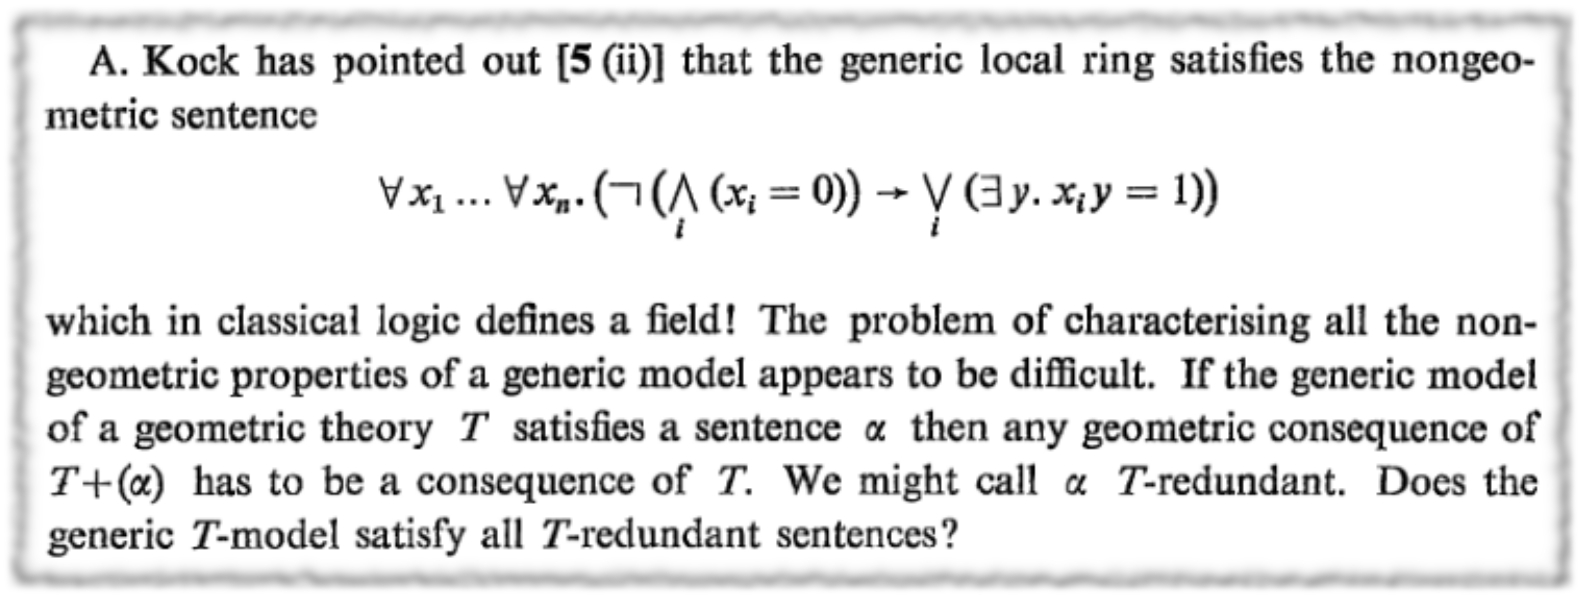
\includegraphics[width=0.9\textwidth]{wraith-some-recent-developments-in-topos-theory} \\
	\scriptsize
        Gavin Wraith. \emph{Some recent developments in topos theory.} \\ In:
        Proc.\@ of the ICM (Helsinki, 1978).
      }
    }};
  \end{tikzpicture}}%

  \[ \xymatrix{
    \text{$\TT$ proves~$\alpha$\;} \ar@/_1pc/@{=>}[r] &
    \text{\;$\alpha$ holds for~$U_\TT$\;} \ar@/_1pc/@{=>}[r]
    \ar@/_1pc/@{=>}@[red][l]
    |{\SelectTips{cm}{}\textbf{\scalebox{3}{\textcolor{red}{\!\texttimes\!}}}}|{} &
    \text{\;$\alpha$ is~$\TT$-redundant}
    \ar@/_1pc/@{=>}@[red][l]
    |{\SelectTips{cm}{}\textbf{\scalebox{3}{\textcolor{red}{\!\texttimes\!}}}}|{}
  } \]
\end{frame}


\section{A topos-theoretic Nullstellensatz}

\newcommand{\nullstellensatz}{%
  \justifying
  \textbf{Theorem.} Internally to~$\Set[\TT]$:

  \begin{quote}\emph{\mbox{For any \explainstub{geometric$^\star$ sequent~$\sigma$}{red!20} over
  the \explainstub{signature of~$\ul{\TT}/U_\TT$}{blue!20},}
  if~\explainstub{$\sigma$ holds for~$U_\TT$}{yellow!70}, then~\explainstub{$\ul{\TT}/U_\TT$
  proves$^\star$~$\sigma$}{yellow!70}.}
  \end{quote}
  \vspace*{-0.6em}
}

\begin{frame}{A topos-theoretic Nullstellensatz}
  \jnote{1-2}{
    By~$\ul{\TT}$ we mean the geometric theory internal to~$\Set[\TT]$ obtained
    by pulling back the set of sorts of~$\TT$, the set of function symbols and so on
    along the unique geometric morphism~$\Set[\TT] \to \Set$. For instance,
    if~$\TT$ is the theory of rings, then from the internal point of view
    of~$\Set[\TT]$, the theory~$\ul{\TT}$ will again be the theory of rings.

    The theory~$\ul{\TT}/U_\TT$ will be defined on the next slide. It is a certain
    geometric theory internal to~$\Set[\TT]$.

    The asterisks in \emph{geometric$^\star$ sequent} and
    \emph{provability$^\star$} indicate that any infinities used to index
    disjunctions have to be come from the base topos. This restriction is an important
    subtlety, though not vital to this talk. If~$\TT$ is a coherent
    theory, then for coherent sequents there is no difference between
    provability in coherent logic, provability in geometric logic and
    provability$^\star$.
  }

  \jnote{2}{
    The algebraic Nullstellensatz states that, in some cases, algebraic truths
    are witnessed by explicit \emph{algebraic certificates} -- syntactical
    objects giving a priori reasons for why a given truth is to be expected.

    In the topos-theoretic Nullstellensatz, algebraic truths are replaced by
    arbitrary truths of the generic model, subject only to the condition that
    they can be expressed as a geometric sequent, and algebraic certificates
    are replaced by \emph{logical certificates}: proofs.
  }

  \jnote{3}{
    While, as stated on slide 1/20, the generic model~$U_\TT$ is a
    conservative~$\TT$-model, the classifying topos~$\Set[\TT]$ does not
    believe this fact. That is, the statement~``$U_\TT$ is a
    conservative~$\ul{\TT}$-model'' is not true internally to~$\Set[\TT]$.
    What is true is the modified statement~``$U_\TT$ is a
    conservative$^\star$~$\ul{\TT}/U_\TT$-model''.
  }

  \nullstellensatz

  \pause

  \textbf{The algebraic Nullstellensatz.}
  Let~$A$ be a ring.
  Let~$f,g \in A[X]$ be polynomials.
  Then, subject to some conditions:
  \[
    \underbrace{\bigl(\forall x \in A\_ (f(x) = 0 \Rightarrow g(x) =
    0)\bigr)}_{\text{algebraic truth}} \Longrightarrow
    \underbrace{\bigl(\exists h \in A[X]\_ g = hf\bigr)}_{\text{algebraic certificate}}
  \]
  \vspace*{-0.9em}

  \pause

  \textbf{A naive version.}
  ``Internally to~$\Set[\TT]$, for any geometric sequent~$\sigma$ over
  the signature of~$\ul{\TT}$,
  if~$\sigma$ holds for~$U_\TT$, then~$\ul{\TT}$
  proves~$\sigma$.'' \textbf{False,} for instance with the theory of rings we
  have
  \begin{align*}
    \Set[\TT] &\models \neg(\speak{$\ul{\TT}$ proves $(\top \vdash 1 + 1 =
    0)$}) \\
    \text{but}\quad \Set[\TT] & \not\models \neg(1 + 1 = 0).
  \end{align*}
\end{frame}

\begin{frame}{A varying internal theory}
  \nullstellensatz

  \explainstub{\textbf{Definition.}}{blue!20} The theory~$\ul{\TT}/U_\TT$ is the
  internal geometric theory of~\hil{$U_\TT$-algebras}, the theory which arises from~$\ul{\TT}$ by adding:
  \begin{enumerate}
    \justifying\small
    \item for each element~$x : U_\TT$ a constant symbol~$e_x$,
    \item for each function symbol~$f$ and~$n$-tuple~$(x_1,\ldots,x_n) \in (U_\TT)^n$ the axiom
    $(\top \vdash f(e_{x_1},\ldots,e_{x_n}) = e_{f(x_1,\ldots,x_n)})$,
    \item for each relation symbol~$R$ and~$n$-tuple~$(x_1,\ldots,x_n) \in (U_\TT)^n$ such
    that~$R(x_1,\ldots,x_n)$ the axiom~$(\top \vdash R(e_{x_1},\ldots,e_{x_n}))$.
  \end{enumerate}

  \textbf{Remark.} Externalising the internal classifying
  topos~$\Set[\TT][\ul{\TT}/U_\TT]$ yields the classifying topos
  of~$\TT$-homomorphisms.

  \jnote{1}{
    Just as locales internal to a topos~$\E$ can be externalised to yield
    localic geometric morphisms into~$\E$, internal Grothendieck toposes can be
    externalised to yield bounded geometric morphisms. Since the composition of
    bounded geometric morphisms is bounded, the externalisation of a
    Grothendieck topos internally to a Grothendieck topos is itself a
    Grothendieck topos, hence the classifying topos of some geometric theory.

    Constructing internally to~$\Set[\TT]$, where~$\ul{\TT}/U_\TT$ is just an
    ordinary geometric theory, the classifying topos of that theory, and then
    externalising the resulting Grothendieck topos results in the classifying
    topos of~$\TT$-homomorphisms. There are two canonical geometric morphisms
    from this topos to~$\Set[\TT]$, the morphism computing the domain and the
    morphism computing the codomain, and the morphism obtained by the
    externalisation procedure is the former.
  }
\end{frame}

\begin{frame}{Revisiting the test cases}
  \nullstellensatz
  \medskip

  \textbf{In the object classifier.}
%  Assume that~$U_\TT$ is empty, that is $\forall x \? U_\TT\_ (\top \Rightarrow
%  \bot)$. By the Nullstellensatz~$\ul{\TT}/U_\TT$ proves~$(\top \seq{x} \bot)$.
%  But this is false in the~$\ul{\TT}/U_\TT$-model~$U_\TT \amalg
%  \{\heartsuit\}$.
  Let~$x,y \? U_\TT$. Assume that~$\neg(x = y)$.
  By the Nullstellensatz~$\ul{\TT}/U_\TT$ proves~$(e_x = e_y \vdash \bot)$.
  But this is false in the~$\ul{\TT}/U_\TT$-model~$U_\TT/(x \sim y)$.
  \medskip

  \textbf{In the ring classifier.}
  Let~$f,g \? U_\TT[X]$ such that any zero of~$f$ is a zero of~$g$.
  By the Nullstellensatz~$\ul{\TT}/U_\TT$ proves this fact.
  Hence it holds in the~$\ul{\TT}/U_\TT$-model~$U_\TT[X]/(f)$. In this
  model~$f$ has the zero~$[X]$. Hence also~$g([X]) = 0$
  in~$U_\TT[X]/(f)$, that is~$g = hf$ for some~$h \? U_\TT[X]$.

  \jnote{1}{
    This slide gives two examples how to use the Nullstellensatz to deduce
    properties of the generic model. A couple of remarks are in order.

    The Nullstellensatz is trivial for sequents~$\sigma$ of the form~$(\top
    \vdash \psi)$. The Nullstellensatz is only interesting in case
    that~$\sigma$ has a nontrivial antecedent or is set in a nonempty context.

    Since the converse direction in the Nullstellensatz also holds
    (because~$U_\TT$ is a~$\ul{\TT}/U_\TT$-model), the
    statements~$\speak{$\sigma$ holds for~$U_\TT$}$
    and~$\speak{$\ul{\TT}/U_\TT$ proves$^\star$ $\sigma$}$ are equivalent. This
    equivalence is intriguing from a logical point of view, since the former
    statement is a geometric implication while the latter can be put as a
    geometric formula. (Up to a subtle issue indicated on the next slide.)

    To apply the Nullstellensatz, no description of a site defining~$\Set[\TT]$
    is required.

    Often when using the Nullstellensatz, we go from an (assumed) truth
    of~$U_\TT$ via provability$^\star$ to another model~$M$
    of~$\ul{\TT}/U_\TT$. That is, we use provability$^\star$ as a (one-way)
    \emph{bridge}:
    \[ \xymatrix{
      & \text{$\ul{\TT}/U_\TT$ proves$^\star$ $\sigma$} \\
      \text{$\sigma$ holds for $U_\TT$} \ar@/^1.1pc/@{<=>}[ur] &&
      \text{$\sigma$ holds for $M$} \ar@/_1.1pc/@{<=}[ul]
    } \]
  }
\end{frame}

{\usebackgroundtemplate{\begin{minipage}{\paperwidth}\vspace*{5.95cm}\hfill\mbox{
\includegraphics[width=0.13\paperwidth]{hen}\;\;}\end{minipage}}
\begin{frame}{Exhaustion and extensions}
  \justifying
  \textbf{Theorem.} A first-order formula holds for~$U_\TT$ iff it is
  intuitionistically provable from the axioms of~$\TT$ and
  the scheme
  \begin{equation}\tag{Nullstellensatz} \speak{$\sigma$ holds} \implies \speak{$\ul{\TT}/U_\TT$
  proves$^{\star\star}$~$\sigma$}. \end{equation}

  \textbf{Theorem.}
  Let~$\TT'$ be a quotient theory
  of~$\TT$. Assume that~$U_\TT$ is contained in the subtopos~$\Set[\TT']$. Then internally
  to~$\Set[\TT']$:
  \begin{quote}
    \emph{A geometric$^\star$ sequent~$\sigma$ with Horn consequent holds for~$U_{\TT'}$
    iff~$\ul{\TT}/U_\TT$ proves$^\star$~$\sigma$.}
  \end{quote}
  \vspace*{-1.6em}

  \textbf{Theorem.}
  % Let~$\mathrm{Form}^\star_{x\?X}(\ul{\TT}/U_\TT)/(\dashv\vdash_{x\?X})$ be the~$\Set[\TT]$-object of
  % geometric$^\star$ formulas over the signature of~$\ul{\TT}/U_\TT$ in the
  % context~$x\?X$, where any two such formulas are identified if and only
  % if~$\ul{\TT}/U_\TT$ proves them equivalent.
  The morphism~$\mathrm{ev}$ is an isomorphism.
  \[ \mathrm{ev} : \mathrm{FunctFormulas}^\star(\ul{\TT}/U_\TT)/(\dashv\vdash)
  \longrightarrow P(U_\TT) \]

  \textbf{Theorem.} A higher-order formula holds for~$U_\TT$ iff it is
  provable in intuitionistic higher-order logic from the axioms of~$\TT$ and
  the higher-order Nullstellensatz scheme.

  \jnote{1}{
    The first theorem states that the source provided by the Nullstellensatz is
    exhaustive. The notion of provability$^{\star\star}$ is a strengthening of
    the notion of provability$^\star$, which in turn is a strengthening of the
    ordinary notion of provability in geometric logic. We are using it here
    because while the notion of provability$^\star$ can be expressed in the
    internal language of a topos, it cannot be expressed in intuitionistic
    logic.

    The second theorem provides a useful variant of the Nullstellensatz. Its
    assumptions are for instance satisfied if~$\TT$ is the theory of rings
    and~$\TT'$ is the theory of local rings. When applicable, it can be used to
    avoid doubly-internal toposes. It also explains, for instance, why in the
    formulation of synthetic quasicoherence no local rings appear even though
    the relevant topos is the classifying topos of local rings.

    The third and fourth theorems generalise the Nullstellensatz to the
    higher-order setting. The map~$\mathrm{ev}$ takes (the equivalence class
    of) a~$\ul{\TT}/U_\TT$-provably$^\star$ geometric$^\star$ formula~$\theta$
    in one free variable to the subset~$\{ x \? U_\TT \,|\, \theta(x) \}$.

    Details on all of this are slowly emerging at
    \fixedhref{https://rawgit.com/iblech/internal-methods/master/paper-qcoh.pdf}{this
    preprint}.
  }

  \jnote{2}{
    XXX future work
  }
\end{frame}}

% Analogy with the harmonic oscillator in the study of physics

% * The generic model
%   * The mystery of nongeometric sequents
%   * Construction of the generic model
% * Kripke--Joyal semantics; focus on existence of extensions
% * Examples for theories and nongeometric sequents with a focus on the wlog
%   aspect
% * Why we are interested in the generic models themselves
%   * Universal localisation
%   * Grothendieck's generic freeness lemma
% * Synthetic quasicoherence
% * Conservativity from the internal point as guiding question
%   * Naive formulation and why it doesn't work
%   * Recall of the algebraic Nullstellensatz
% * The new Nullstellensatz
%   * What Set[T][T/U_T] classifies
%   * Kock again
%   * Subtleties regarding infinites
%   * Improvement in the Horn case
% * Universality of the source provided by the Nullstellensatz

\end{document}


% Are there size issues when KJ'ing internally?
% Comparison to the approach by Vickers?
% When does a theory prove the Nullstellensatz?
% Look up what Kock and Reyes used the wlog for.

% An Tafel: geometric formula, local ring
% Erwähnen: Marc Bezem, Ulrik Buchholtz, Thierry Coquand

% Grothendieck quote for the title picture:
%
% Ces “nuages probabilistes”, remplaçant les rassurantes particules matérielles
% d’antan, me rappellent étrangement les élusifs “voisinages ouverts” qui
% peuplent les topos, tels des fantômes évanescents, pour entourer des “points”
% imaginaires, ...
%
% Diese "Wahrscheinlichkeitswolken", welche die beruhigenden materiellen
% Partikel von früher ersetzen, erinnern mich irgendwie an die flüchtigen
% "offenen Umgebungen" der Topoi -- wie dahinschwindende Phantome, um
% die fiktiven "Punkte" zu umgeben, ...
%
% These “probability clouds”, replacing the reassuring material particles of
% before, remind me strangely of the elusive “open neighborhoods” that populate
% the topoi, like evanescent phantoms, to surround the imaginary “points”.

% Sei T eine Theorie, für die ein konservatives Modell in Set existiert.
% Dann haben wir eine Surjektion Set --> Set[T]. Also existiert eine
% geometric expansion von T, welche Morita-äquivalent zur leeren Theorie ist.
